    %   Il progetto nasce dal template per il frontespizio realizzato da Marco Antonio Corallo, che ringrazio. Seguono alcuni commenti per evidenziare la presenza di alcuni pacchetti che mi sono stati utili per la stesura della tesi. Chiaramente, dipende tutto dal tipo di lavoro che uno vuole eseguire, che determina anche le diverse esigenze. Durante la stesura ho passato molto tempo su siti e forum a cercare di risolvere alcuni probelmi di formattazione, ma in generale Latex è stato piuttosto versatile. 

% Tipo di documento. L'uso di twoside implica che i capitoli inizino sempre con la prima pagina a sinistra, eventualmente lasciando una pagina vuota nel capitolo precedente. Se questa cosa è fastidiosa, è possibile rimuoverlo. 
\documentclass[a4paper, twoside,openright]{article}

\usepackage{enumerate}% http://ctan.org/pkg/enumerate
% Dimensione dei margini
\usepackage[a4paper,top=3cm,bottom=3cm,left=3cm,right=3cm]{geometry} 
% Dimensione del font
\usepackage[fontsize=11pt]{scrextend}
% Lingua del testo
\usepackage[english]{babel}
% Lingua per la bibliografia
\usepackage[fixlanguage]{babelbib}
% Codifica del testo
\usepackage[utf8]{inputenc} 
% Encoding del testo
\usepackage[T1]{fontenc}
% Permette di generare testo fittizio. Mi è stato utile 
% per capire quale sarebbe stata l'impostazione del 
% testo nella pagina prima che scrivessi un determinato paragrafo
\usepackage{lipsum}
% Per ruotare le immagini
\usepackage{rotating}
% Per modificare l'header delle pagine 
\usepackage{fancyhdr}         

% Librerie matematiche
\usepackage{amssymb}
\usepackage{amsmath}
\usepackage{amsthm}         
% Uso delle immagini
\usepackage{graphicx}
% Uso dei colori
\usepackage[dvipsnames]{xcolor}         
% Uso dei listing per il codice
\usepackage{listings}          
% Per inserire gli hyperlinks tra i vari elementi del testo 
\usepackage{hyperref}     
% Diversi tipi di sottolineature
\usepackage[normalem]{ulem}

\usepackage{array}
\usepackage{float}
\usepackage{subcaption}

% Modifica lo stile dell'header
\pagestyle{fancy}
\fancyhf{}
\lhead{\leftmark}
\rhead{\textbf{\thepage}}
\fancyfoot{}
\setlength{\headheight}{14pt}
% Rimuove il numero di pagina all'inizio dei capitoli
\fancypagestyle{plain}{
  \fancyfoot{}
  \fancyhead{}
  \renewcommand{\headrulewidth}{0pt}
}

% Stile del codice
\lstdefinestyle{codeStyle}{
    % Colore dei commenti
    commentstyle=\color{teal},
    % Colore delle keyword
    keywordstyle=\color{Magenta},
    % Stile dei numeri di riga
    numberstyle=\tiny\color{gray},
    % Colore delle stringhe
    stringstyle=\color{violet},
    % Dimensione e stile del testo
    basicstyle=\ttfamily\footnotesize,
    % newline solo ai whitespaces
    breakatwhitespace=false,     
    % newline si/no
    breaklines=true,                 
    % Posizione della caption, top/bottom 
    captionpos=b,                    
    % Mantiene gli spazi nel codice, utile per l'indentazione
    keepspaces=true,                 
    % Dove visualizzare i numeri di linea
    numbers=none,                    
    % Distanza tra i numeri di linea
    numbersep=5pt,                  
    % Mostra gli spazi bianchi o meno
    showspaces=false,                
    % Mostra gli spazi bianchi nelle stringhe
    showstringspaces=false,
    % Mostra i tab
    showtabs=false,
    % Dimensione dei tab
    tabsize=2
} \lstset{style=codeStyle}


% Stile di codice per dimensioni maggiori, in cui ho avuto bisogno di un testo più picolo (ad esempio se si vuole inserire del codice che ha linee molto lunghe). Per usare questo stile piuttosto che il precedente, usare 

% \lstset{style=longBlock}
%  % inserire il codice...
% \lstset{style=codeStyle}

% Il secondo comando consente di tornare allo stile precedente 
\lstdefinestyle{longBlock}{
    commentstyle=\color{teal},
    keywordstyle=\color{Magenta},
    numberstyle=\tiny\color{gray},
    stringstyle=\color{violet},
    basicstyle=\ttfamily\scriptsize,
    breakatwhitespace=false,         
    breaklines=true,                 
    captionpos=b,                    
    keepspaces=true,                 
    numbers=left,                    
    numbersep=5pt,                  
    showspaces=false,                
    showstringspaces=false,
    showtabs=false,                  
    tabsize=2
} \lstset{style=codeStyle}

% Togliendo il commento al comando che segue, si inseriscono nella bibliografia anche le fonti presenti in Bibliography.bib ma non citati direttamente con il comando \cite
% \nocite{*}

% Margini prima e dopo blocchi di codice, per avere più distanza
\lstset{aboveskip=20pt,belowskip=20pt, morekeywords={PK, FK, ref, on}}

% Modifica dello stile dei riferimenti, con il testo in cyano
\hypersetup{
    colorlinks,
    linkcolor=Black,
    citecolor=Black
}

% Aggiunti definizioni, teoremi, linea e listing
\newtheorem{definition}{Definizione}[section]
\newtheorem{theorem}{Teorema}[section]
\providecommand*\definitionautorefname{Definizione}
\providecommand*\theoremautorefname{Teorema}
\providecommand*{\listingautorefname}{Listing}
\providecommand*\lstnumberautorefname{Linea}

%\raggedbottom

%\newcommand{\cgs}[1]{{\textcolor{brown}[\textcolor{red}{\bf{GS: }}{ \textcolor{brown}{#1]}}}}             
%\newcommand{\cmc}[1]{{\textcolor{blue}[\textcolor{magenta}{\bf{MC: }}{ \textcolor{blue}{#1]}}}}

\newcolumntype{M}[1]{>{\centering\arraybackslash}m{#1}}


% -----------------------------------------------------------------
\begin{document}

\begin{titlepage}
\begin{figure}[!htb]
    \centering
    
\includegraphics[keepaspectratio=true,width=0.4\textwidth]{images/Frontespizio/stemma.pdf}
\end{figure}

\begin{center}
    \LARGE{\bf UNIVERSITY OF FLORENCE}
    \vspace{5mm}
    \\ \large{Department of Information Engineering}
    \vspace{5mm}
    \\ \large{Master Degree in Information Engineering}
\end{center}

\vspace{12mm}
\begin{center}
    {\LARGE{\bf Project report of Quantitative Evaluation of Stocastic Models and Software Architecture and Metodologies}} \\
    {\large \textit{Predictive autoscaling using stocastic models for Kubernetes}}
    % Se il titolo è abbastanza corto da stare su una riga, si può usare
    
    % {\LARGE{\bf Un fantastico titolo per la mia tesi!}}
\end{center}
\vspace{28mm}

\begin{minipage}[t]{0.47\textwidth}
	{\large{Lecturer:}{\normalsize\vspace{3mm}
	\bf\\ \large{Prof. Vicario Enrico} \normalsize\vspace{3mm}\bf }}
\end{minipage}
\hfill
\begin{minipage}[t]{0.47\textwidth}\raggedleft
	{\large{Students:}{\normalsize\vspace{3mm} \bf\\ \large{Beragnoli Jacopo}\normalsize\vspace{3mm} \\ \large{Lucchesi Carlo}\normalsize\vspace{3mm}\\ \large{Orsucci Giacomo} \normalsize\vspace{3mm} \negthickspace \!}}
\end{minipage}

\vspace{27mm}
\hrulefill
\\\centering{\large{Academic Year 2024/2025}}

\end{titlepage}
\include{chapters/Abstract}

\tableofcontents

\section{Introduction}
 

\subsection{Statement}

We want to build a micro-service oriented architecture using Kubernetes (K8s) to deploy and scale horizontally our containers (pods in K8s terminology). The goal of the project is to create a complete platform to study the behaviors and the increased capacities of an horizontal scaling based on a message-queue rejection rate. In doing so, technologies such as K6, RabbitMQ, Kafka, Docker, Grafana, Prometheus and Sirio Framework will be used. In details, we want to models different types of load (Poisson, Uniform, Erlang inter arrival times) with different rates to generate messages. Exploiting information about the arrival, we use a stochastic model of the system to recommend horizontally scaling of service's pods, in order to meet a rejection rate target. 

\subsection{Project goal and working environment}
The goal of the project is to verify the feasibility and efficacy of a horizontal autoscaler based on stochastic properties of the model that represent a queue system. Using the framework Sirio it is possible to define Stochastic Time Petri Nets that models the behavior of a microservices system, and evaluate some quantity of interest (like Rejection Rate). The objective is to scale the number of services in the most efficient way while respecting a Service Level Agreement (SLA), identified in this case as a maximum rejection rate tolerated. The working environment is developed using Kubernetes and consists of these main components:
\begin{itemize}
    \item \textbf{Arrival Service}: this service generates the requests following a particular stochastic distribution. This is implemented using K6 tool.

    \item \textbf{K6}: a framework used to stress test systems like ours.

    \item \textbf{Queue}: this element buffers the requests, allowing the worker to elaborate them in a second moment. We decided to use RabbitMQ for the main queue thanks to the provided possibility of setting the queue size explicitly.

    \item \textbf{Process Service:} this service pulls messages from the queue and elaborates them. We did a custom implementation in Pyhton that simply executes a busy wait.
    
    \item \textbf{Monitoring/Visualization:} it’s done using Prometheus as metric server, in combination with Grafana for the dashboards.

    \item \textbf{Sirio Controller:} this Java service utilizes the CDF of the arrival process (calculated using another custom service) to build a STPN and evaluating the rejection rate. Then, it recommends to Kubernetes the minimum number of active replicas needed to respect the SLA.
    
\end{itemize}

\clearpage

\section{System design}
\subsection{C4 model} \label{sec:ucdiagram}


This project adopts a structured approach to software architecture documentation based on the C4 model, a hierarchical visualization framework that enables clear communication of complex system architectures. The documentation is organized through four distinct levels of abstraction: software systems, containers, components, and code, each serving specific communication needs and technical depth requirements. The C4 model provides a lean graphical notation technique for modeling software system architectures through structural decomposition.
\begin{itemize}
    \item \textbf{Level 1 - Software Systems:} The highest level of abstraction describing systems that deliver value to users, whether human or automated. A software system represents something a single development team builds, owns, and has responsibility for, typically corresponding to team boundaries and deployment units.

    \item \textbf{Level 2 - Containers:} Runtime applications or data stores that must be running for the overall system to function. These include services, APIs, and message queues - essentially the major building blocks that distribute system responsibilities.

    \item \textbf{Level 3 - Components:} Internal elements within each container, showing how components interact with each other and external systems. This level reveals the logical groupings and interfaces that compose each container's functionality.

    \item \textbf{Level 4 - Code:} The most detailed view showing classes, interfaces, and code-level relationships.

\end{itemize}
This chapter will present and describe the C4 diagrams that have been developed.
\subsection{Level 1 - Software Systems}
\begin{figure}[H]
    \centering
    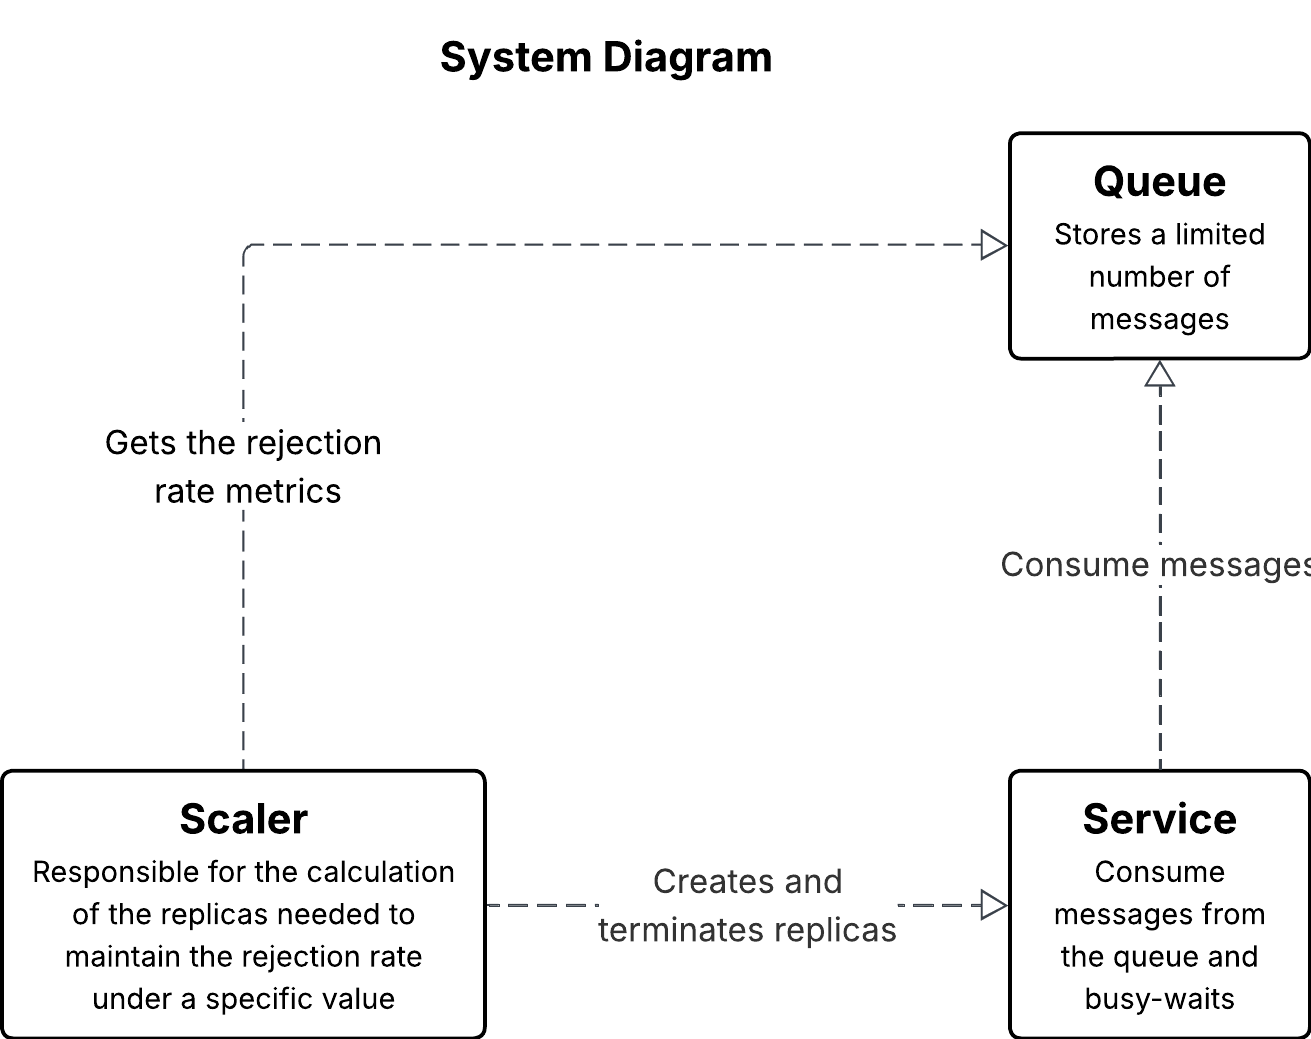
\includegraphics[width=0.75\linewidth]{images/C4 model/SystemDiagram.png}
    \caption{System Diagram}
    \label{fig:system_diagram}
\end{figure}

As shown in the Figure, the level 1 represents the highest level of abstraction of our system and it highlights its major components and functionalities. Its core comprehends a queue (reached by the messages generated) from which are exposed the necessary metrics to scale our service in order to achieve the chosen SLA. 

\subsection{Level 2 - Containers}

\begin{figure}[H]
    \centering
    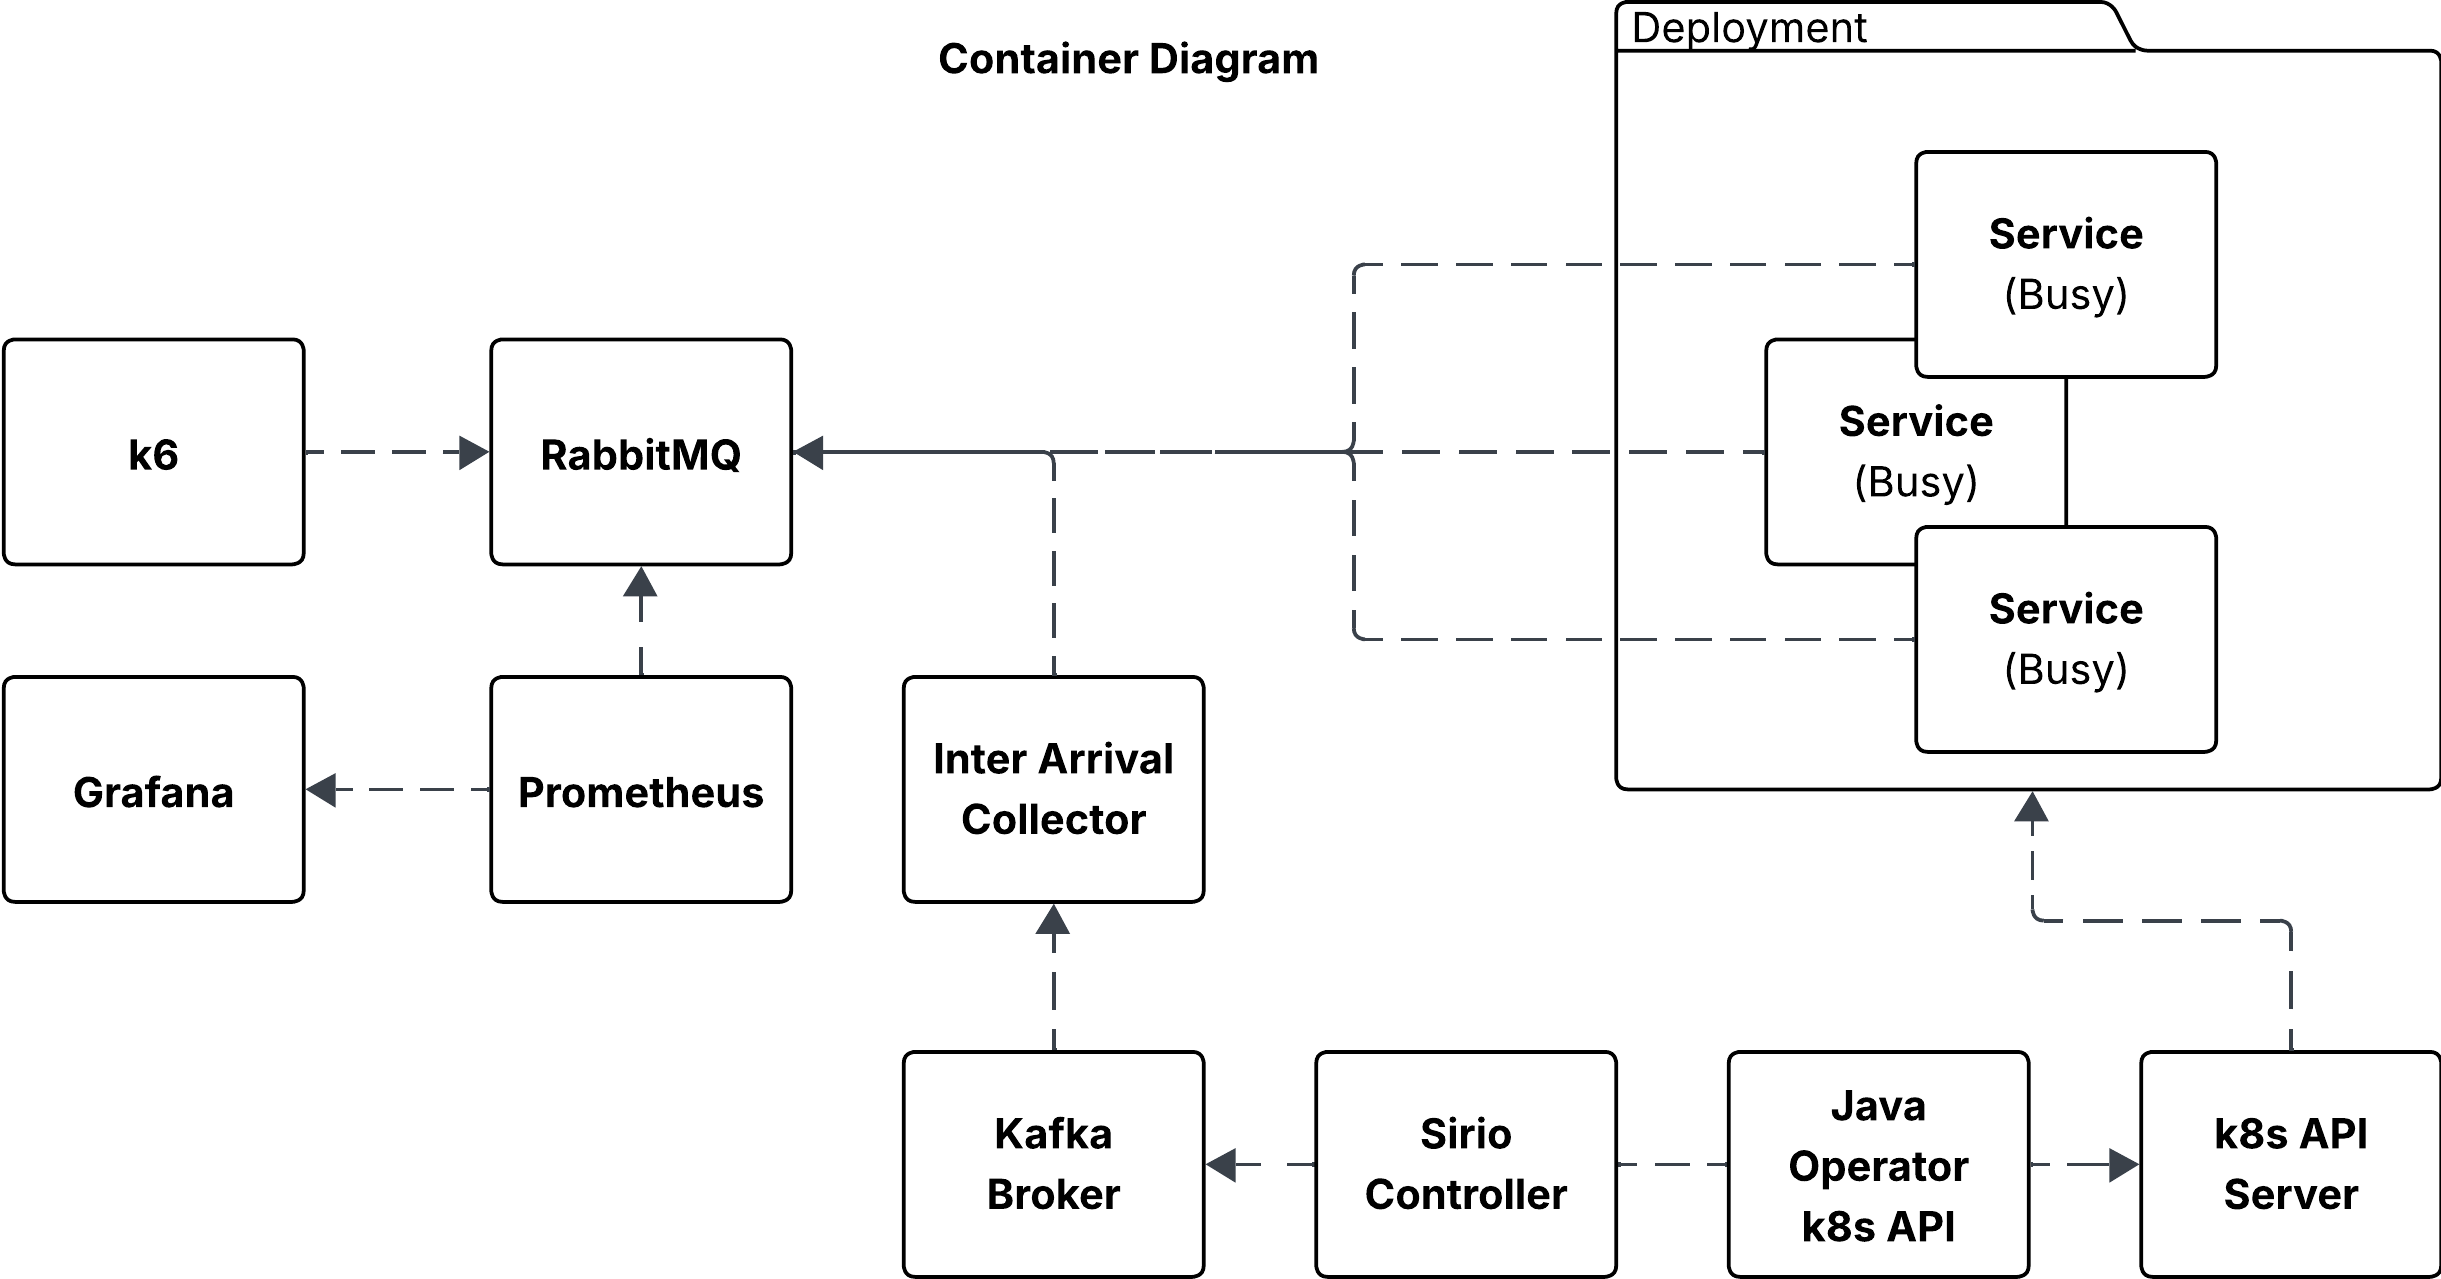
\includegraphics[width=0.75\linewidth]{images/C4 model/ContainerDiagram.png}
    \caption{Container Diagram}
    \label{fig:container_diagram}
\end{figure}


Going more in depth we see the container organization, which allows us to detail all the micro services built and their functions. Starting from left we have k6 to generate the load (in our case modeled as a state machine). The messages are stored in a RabbitMQ queue, which exposes the metrics of our interest on Grafana via Prometheus and to the Inter Arrival Collector. The Inter Arrival Collector exposes the CDF messages (with the CDF calculated on the interarrivals from the queue) on a Kafka broker that passes the messages to the Sirio Controller component, that uses the CDFs to estimate via the internal model the rejection rate. The number of replicas are estimated to keep the rejection rate under the target fixed. On the basis of this estimate, the kubernetes API is used to scale the services horizzontally (their number is increased or decreased).


\subsection{Level 3 - Components}
At the component architecture level, we have implemented a series of containers, entirely contained within the \verb|oris-predictive-autoscaler| namespace (ns). The architecture is divided into three main logical areas:
\begin{enumerate}
    \item The \textbf{System Under Test (SUT)}, which includes the custom applications and the basic messaging infrastructure (Kafka and RabbitMQ).
    \item The \textbf{Accessory Monitoring Services}, which provide observability and workload analysis capabilities.
    \item The \textbf{Security and Access Control (RBAC)} configuration, which governs the permissions of the various components within the cluster.
\end{enumerate}

\subsubsection{System Under Test (SUT)}
The SUT represents the core of the system and includes both the custom-developed application components (yellow background) and the infrastructure services they rely on (white background).
Asynchronous communication and data flow management are handled by two message brokering systems:
\begin{itemize}
\item \textbf{rabbitmq}: The message broker, used as the incoming request queue for the service. It is also implemented as a \textbf{StatefulSet (sts)} and configured via two \textbf{ConfigMaps (cm)}: \verb|rabbitmq-definitions| and \verb|rabbitmq-config|, which define its policies, queues, and initial settings. A \textbf{Service (svc)} ensures its accessibility.
    \item \textbf{kafka}: Used as a notification and data exchange system between the \verb|inter-arrival-collector| and the \verb|sirio-controller|. Being a stateful system, it is implemented as a \textbf{StatefulSet (sts)} to ensure stable network identities and persistent storage, managed via a \textbf{PersistentVolumeClaim (pvc)}. A \textbf{Service (svc)} exposes Kafka within the cluster, allowing components to communicate with it.

\end{itemize}

\subsubsection{Custom Services}
These are the components where the specific business logic of the autoscaling system resides.
\begin{itemize}
    \item \textbf{sirio-controller}: Contains the \verb|sirio-controller| \textbf{Deployment}, which represents the brain of the system. This controller implements the predictive autoscaling logic, monitoring metrics and making decisions on how and when to scale the service. The deployment's code diagram will be presented in the next chapter, \ref{sec:code}.
    \item \textbf{inter-arrival-collector}: This \textbf{Deployment} is responsible for collecting the inter-arrival times of requests. Acquiring this data is fundamental for the predictive model. Once collected, the data is sent to Kafka to be processed by the \verb|sirio-controller|.
    \item \textbf{python-service}: This \textbf{Deployment} represents the target application, i.e., the service that is monitored and whose number of replicas is dynamically managed by the \verb|sirio-controller|.
\end{itemize}

\subsubsection{Operations and Monitoring}
These services (green background) are not part of the main application logic (SUT) but are crucial for collecting metrics, analyzing performance, and visualizing the system's state.

\begin{itemize}
    \item \textbf{prometheus}: It is the central monitoring and alerting system. Implemented as a \textbf{Deployment}, it uses a \textbf{ConfigMap} (\verb|prometheus-config|) to define the targets from which to scrape metrics (such as \verb|kube-state-metrics| and the SUT applications). A \textbf{Service} exposes its interface so that it can be easily reached by Grafana.
    \item \textbf{kube-state-metrics}: An essential service that connects to the Kubernetes API Server to generate metrics about the state of cluster objects (in this case, the number of pods in a deployment). These metrics are then collected by Prometheus to be displayed on Grafana.
    \item \textbf{grafana}: A visualization tool that connects to Prometheus as a datasource. Its \textbf{Deployment} is configured via two \textbf{ConfigMaps}: \verb|grafana-datasource| to set up the connection to Prometheus and \verb|grafana-dashboards| to preload custom dashboards. 
\end{itemize}

 \begin{figure}[ht]
    \centering
    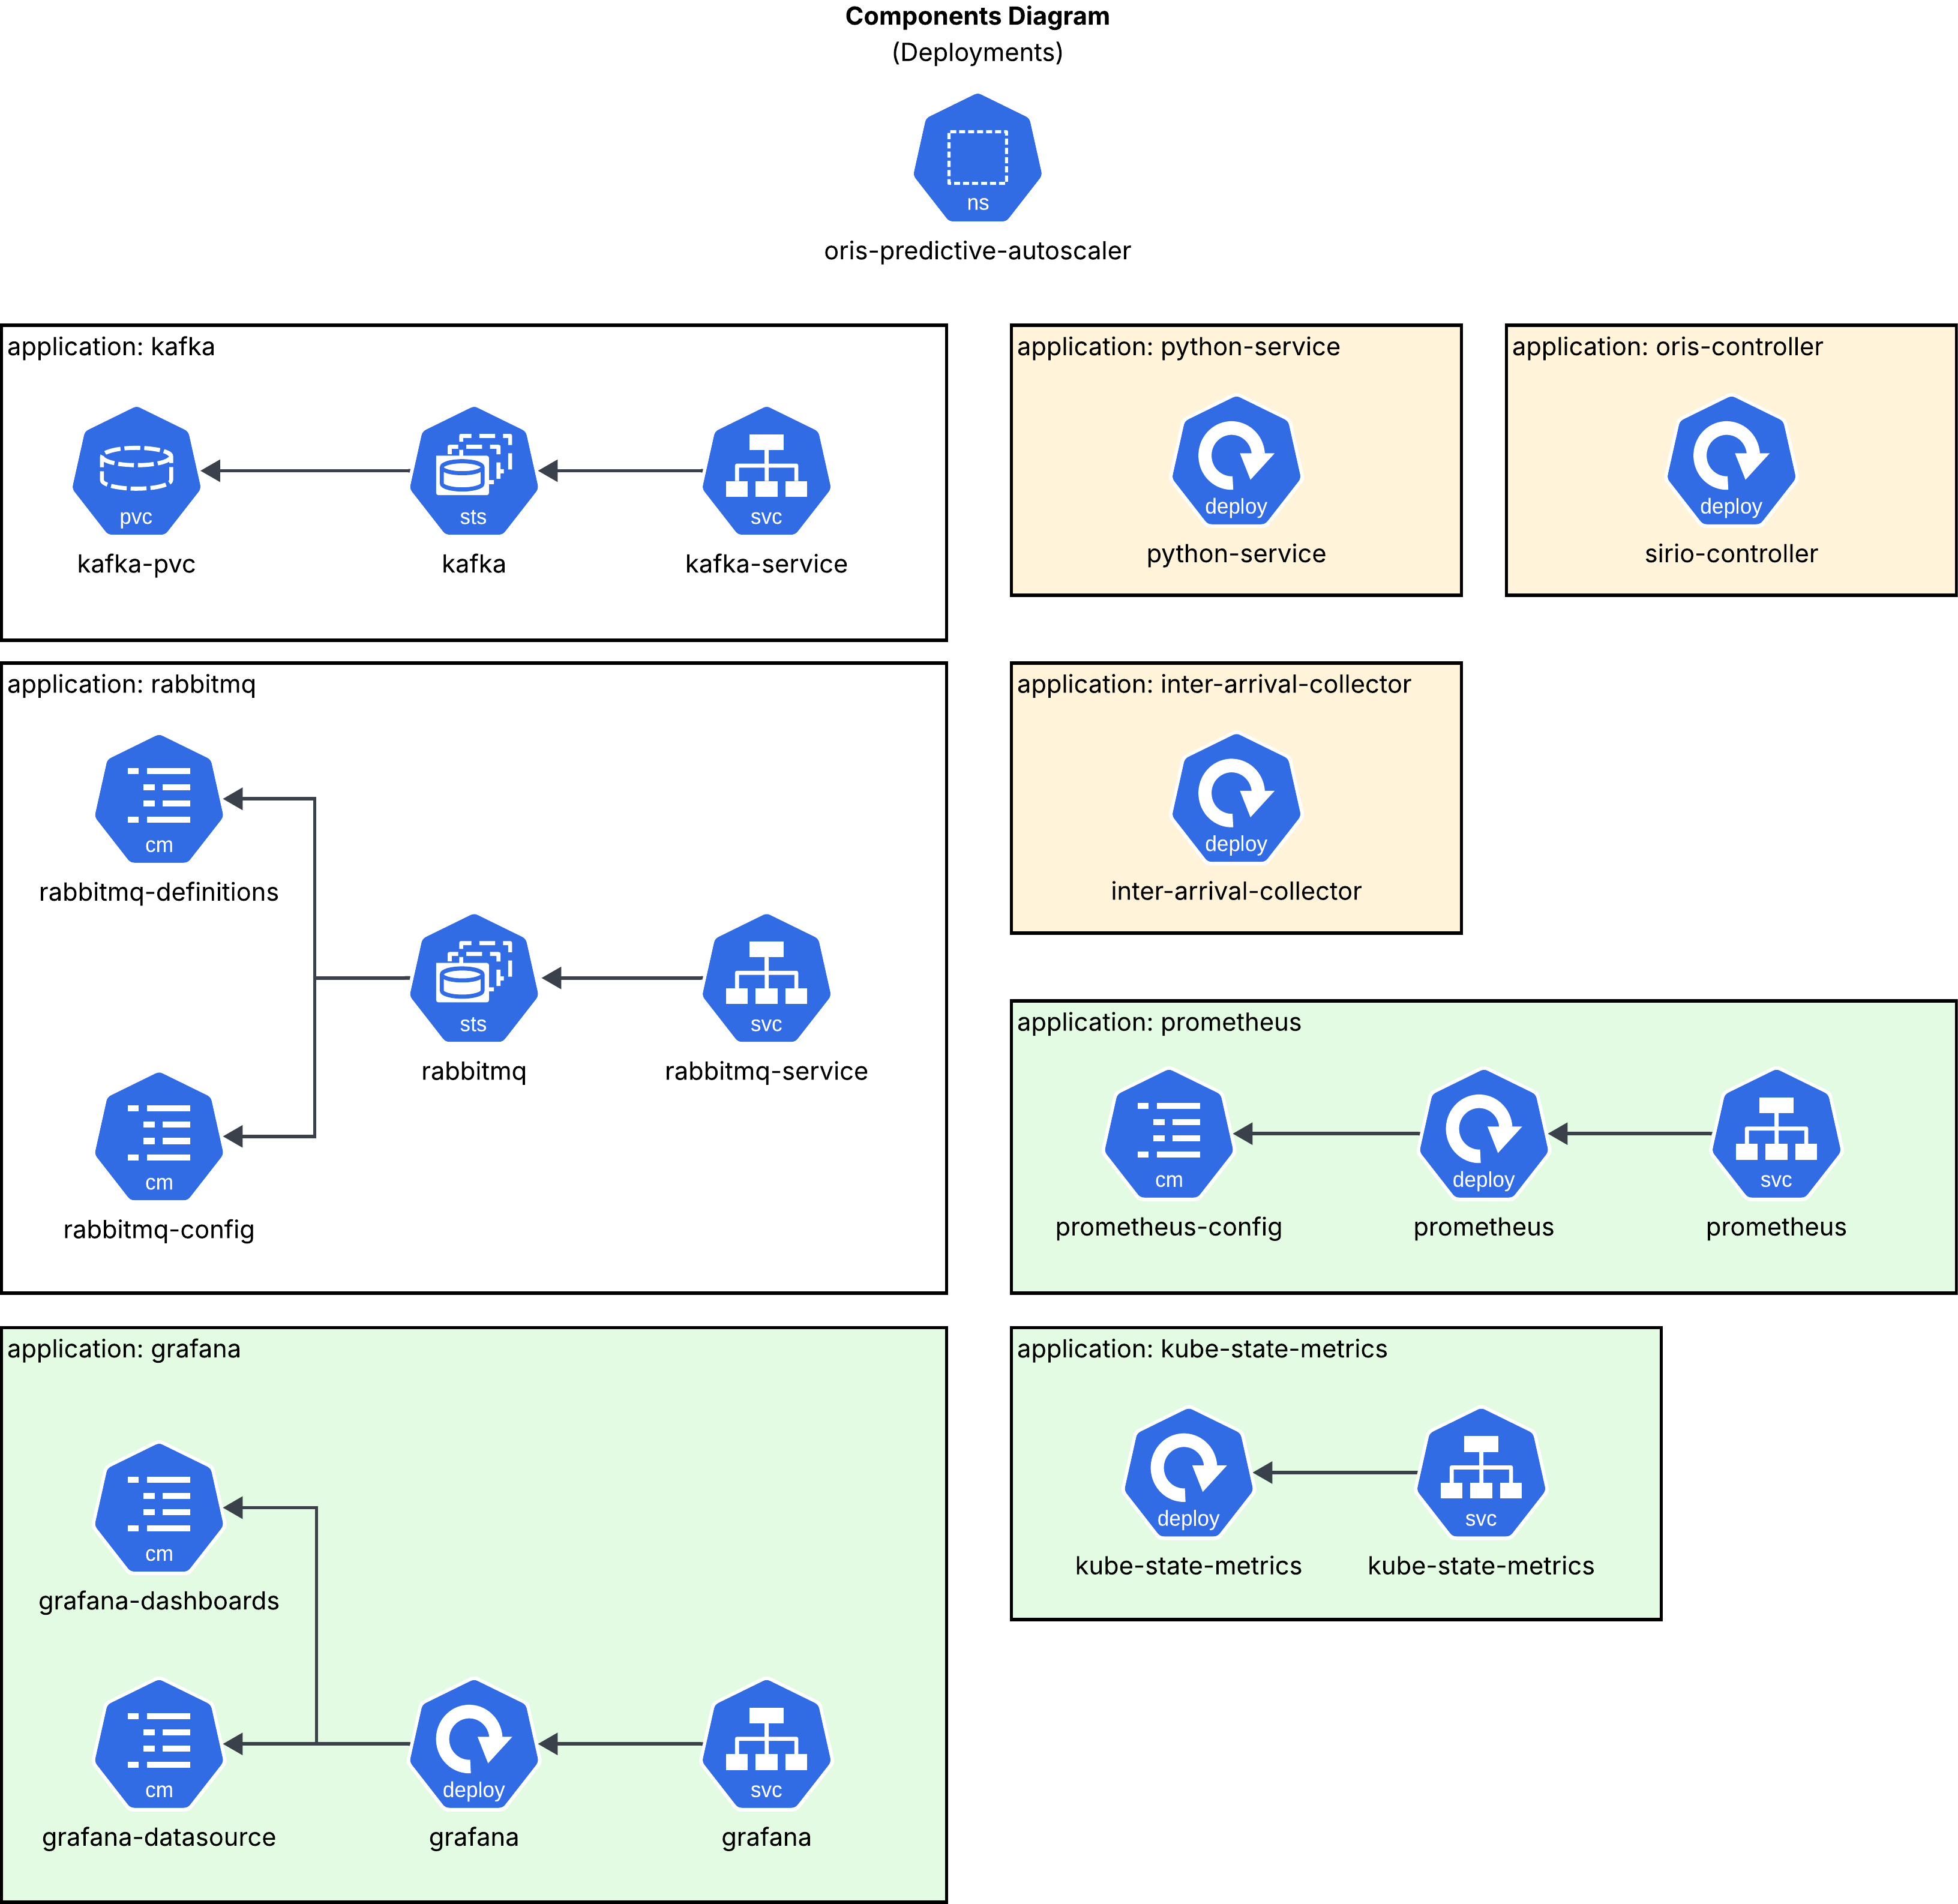
\includegraphics[width=0.75\linewidth]{images/C4 model/componentDiagram_deploy.png}
    \caption{Deployments Diagram}
    \label{fig:component_diagram_deploy}
\end{figure}

\subsubsection{Role-Based Access Control}
 The second diagram illustrates the RBAC (Role-Based Access Control) configurations that ensure each component operates on the principle of least privilege, accessing only the resources that are strictly necessary.

\begin{itemize}
    \item \textbf{kube-state-metrics-rbac}: In order to generate metrics on the entire cluster, this service needs read permissions on all Kubernetes objects. Its configuration includes:
    \begin{itemize}
        \item A \textbf{ServiceAccount (sa)}: \verb|kube-state-metrics|, the identity used by the pod.
        \item A \textbf{ClusterRole (c.role)}: Defines \verb|get|, \verb|list|, \verb|watch| permissions at the cluster level.
        \item A \textbf{ClusterRoleBinding (crb)}: Binds the \verb|ClusterRole| to the \verb|ServiceAccount|, making the permissions effective.
    \end{itemize}
    \item \textbf{sirio-controller-rbac}: Being the heart of the autoscaling logic, the controller must be able to monitor and modify the state of other objects (like Deployments). In this case as well, the configuration uses a \textbf{ServiceAccount}, a \textbf{ClusterRole}, and a \textbf{ClusterRoleBinding} to grant it the necessary permissions to operate at the cluster scale.
    \item \textbf{prometheus-operator-rbac}: This is the most complex configuration because it deals with defining the functionalities and permissions of the Prometheus Operator. The operator requires permissions at both the namespace and cluster levels:
    \begin{itemize}
        \item A \textbf{Role} and a \textbf{RoleBinding (rb)}: grant it specific permissions within the \verb|oris-predictive-autoscaler| namespace.
        \item A \textbf{ClusterRole} and a \textbf{ClusterRoleBinding (crb)}: grant it broader permissions, necessary to discover services to monitor across the entire cluster or to manage resources globally.
    \end{itemize}
\end{itemize}

\begin{figure}[ht]
    \centering
    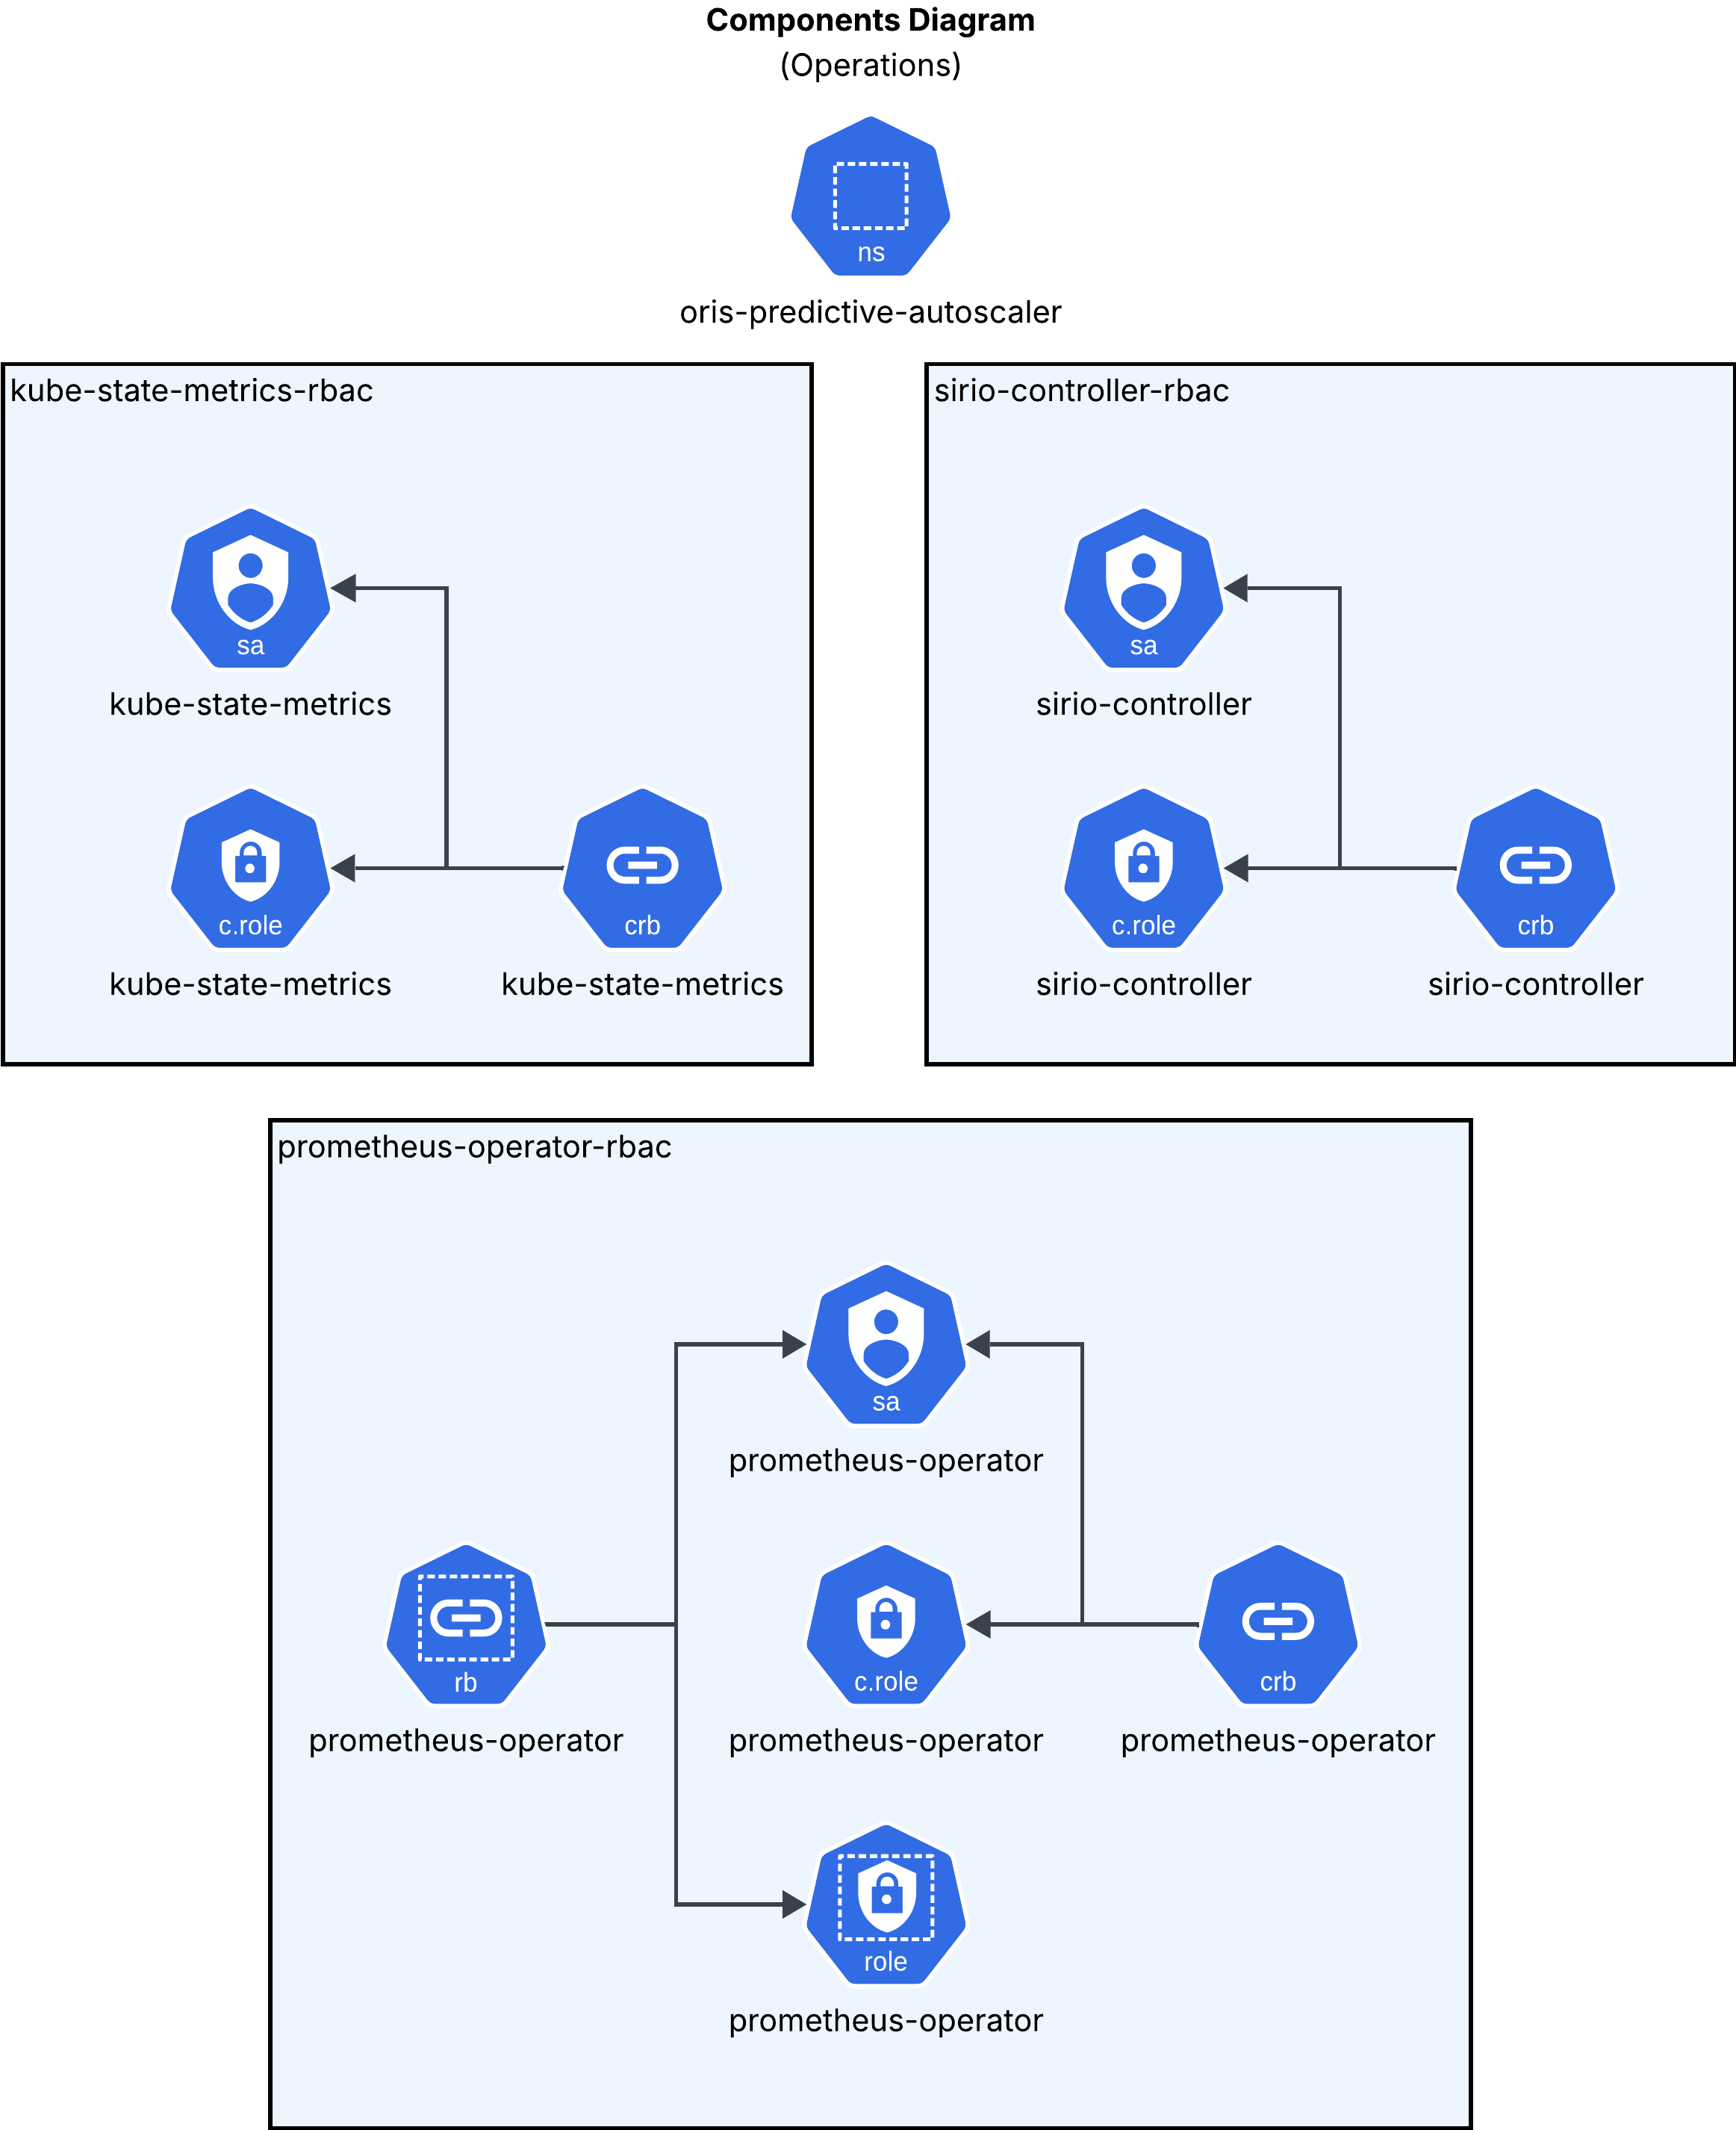
\includegraphics[width=0.75\linewidth]{images/C4 model/componentDiagram_operations.png}
    \caption{Operations Diagram}
    \label{fig:uccomponent_diagram_operations}
\end{figure}
\newpage
\subsection{Level 4 - Code} \label{sec:code}
And finally, the code:

\begin{figure}[H]
    \centering
    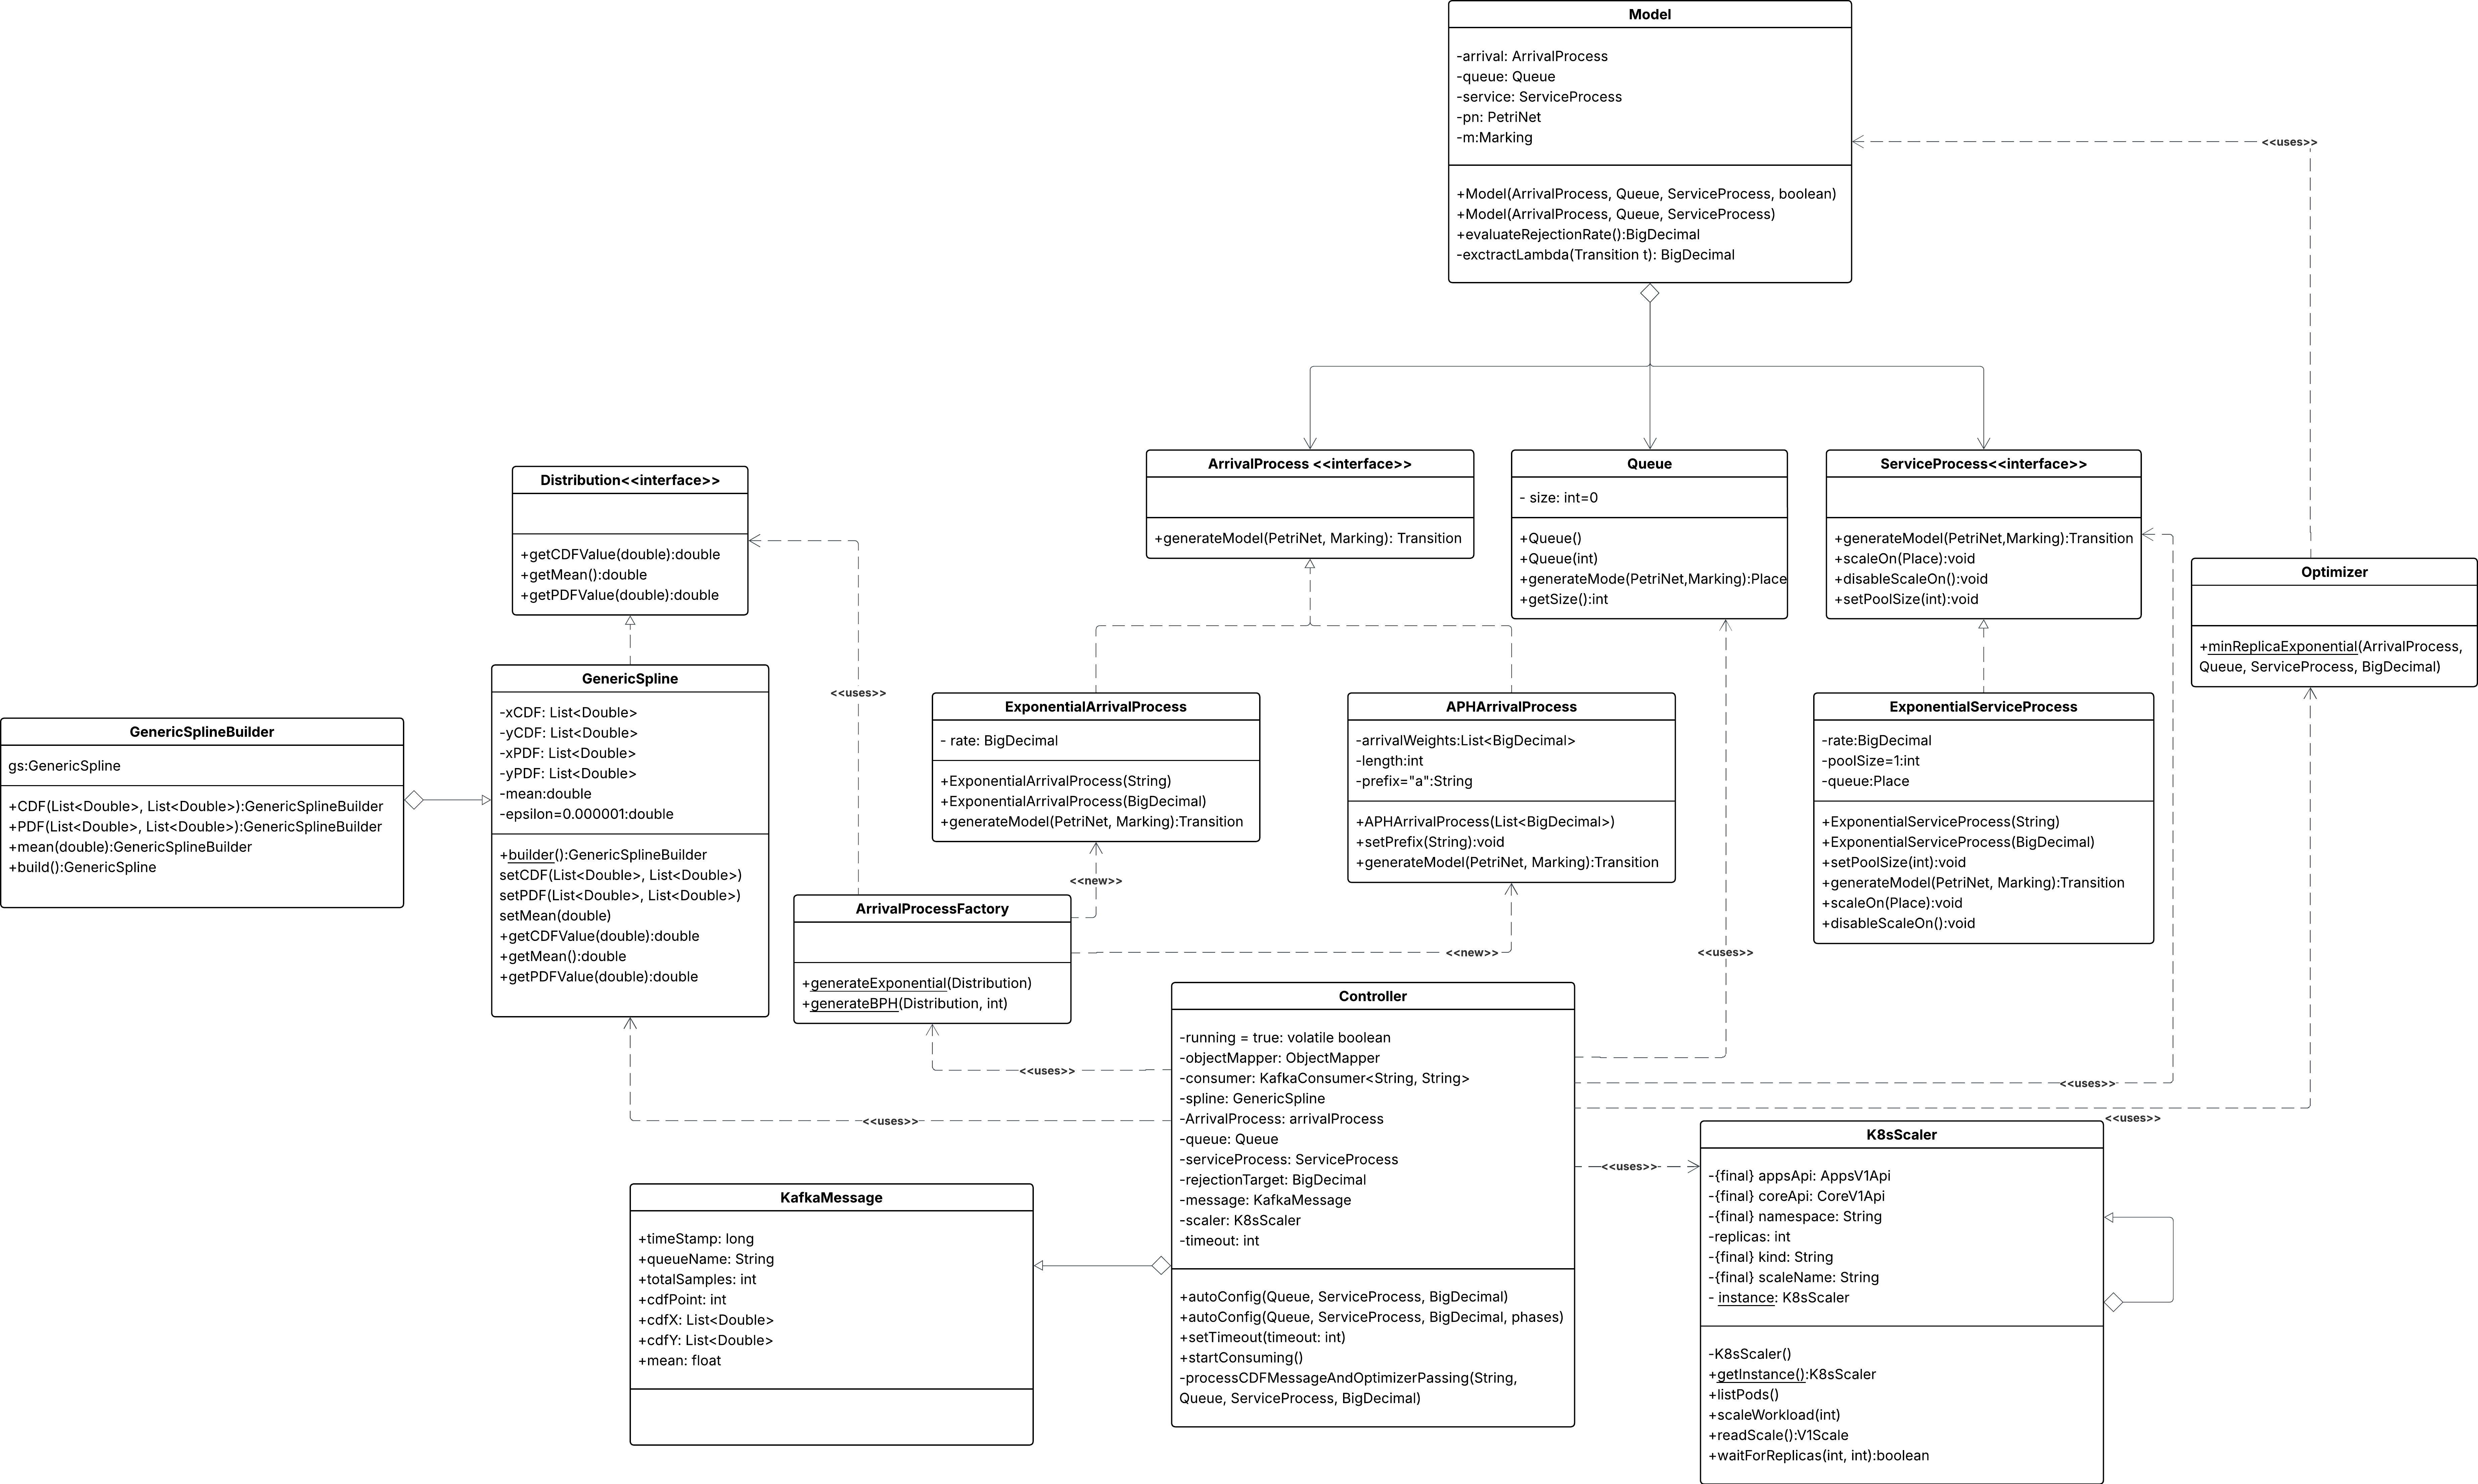
\includegraphics[width=1\linewidth]{images/C4 model/UML.png}
    \caption{UML Class Diagram}
    \label{fig:uml_diagram}
\end{figure}

This is the UML class diagram for the Sirio controller. What is good to note is that it is the piece of code to construct the model and evaluate the rejection rate constructing a real model of the problem and using the CDF received and mapped in the KafkaMessage class. All things considered, the core of this code is the optimizer because it uses all the other elements to iteratively evaluate the rejection rate for an increasing number of replicas. When the best number is found, the scaler is commanded. Follow \href{https://lucid.app/lucidchart/5c1b70c3-c1c8-470e-b04a-fefab525a1fc/edit?invitationId=inv_05163187-b3ea-4a1a-a14b-3cdabad1d3d5&page=XRAN4fSOEXo6#}{this link} for a better visualization.
\section{Experiments}

\subsection{Machine Specification}
We executed the following tests using this environment:

%TODO Please Bera write down your machine spec.

\begin{itemize}
    \item \textbf{Machine}:
    \begin{itemize}
        \item Type:
        \item CPU: 
        \item RAM: 
    \end{itemize}
    \item \textbf{Software}:
    \begin{itemize}
        \item OS: 
        \item Kubernetes: 
    \end{itemize}
\end{itemize}

\subsection{Experiments Description}
The experiments have the goal of emulating different types of traffic, with the objective of showing the system behavior. The possible experiments can be performed choosing different rates following a state machine. In other words, if the user selects 4 different rates for the distribution selected the load is composed of 4 circularly executed states with the rated specified. The duration of each state is editable from the code.

So, for example, choosing a uniform distribution with all rates value such that min=max (to model the deterministic arrival process) and selecting a test with a duration of 9 minutes and rates = ([1,1];[2,2];[3,3];[5,5]) we are modelling an arrival process that generates a load with 1 message/s for 1 minute, than 2 messages/s for 1 minute, than 3 messages/s for 1 minute, than 5 messages/s for 1 minute. At this point 4 minutes has been passed so the arrival process restarts circularly from 1 message/s and so on until the end of the test.

\subsection{Experiments guide}
In this section we include a miniguide to reproduce our experiments. First of all it is necessary to clone the GitHub repository at \href{https://github.com/Berags/oris-predictive-autoscaler}{this link} (https://github.com/Berags/oris-predictive-autoscaler). To start the project is necessary, as a minimum dependancy, to have installed \href{https://minikube.sigs.k8s.io/docs/}{Minikube}. After having installed successfully Minikube, execute the following command:

\begin{table}[!htb]
\centering
\begin{tabular}{c}
\begin{lstlisting}
minikube start
\end{lstlisting}
\end{tabular}
\end{table}

then, it is sufficient to position the terminal on the directory of the project where it is present the .sh file named ./start.sh and execute:

\begin{table}[!htb]
\centering
\begin{tabular}{c}
\begin{lstlisting}
./start.sh
\end{lstlisting}
\end{tabular}
\end{table}
the file start.sh contains all the instruction necessary to build and run our project (i.e. all the containers and components). Don't mind if it takes a while, it is perfectly normal due to the project complexity. At this point, as reported in \guillemotleft port-forward.sh\guillemotright \ you can monitor:
\begin{itemize}
  \item The RabbitMQ queue at \guillemotleft http://localhost:15672\guillemotright
  \item Prometheus at \guillemotleft http://localhost:9090\guillemotright
  \item Grafana (with all the dashboards of interest shown below) at \guillemotleft http://localhost:3000\guillemotright, the default username and password is \verb|admin|.
  \item Kafdrop (for the Kafka queue) at \guillemotleft http://localhost:9000\guillemotright
\end{itemize}

At this point everything is ready to start the tests. In order to do it, go ( we suggest with an additional terminal window) in the folder of \guillemotleft build-and-run.sh\guillemotright \ that is inside the \guillemotleft k6 \guillemotright folder and execute the file with
\begin{table}[!htb]
\centering
\begin{tabular}{c}
\begin{lstlisting}
./build-and-run.sh
\end{lstlisting}
\end{tabular}
\end{table}

\begin{lstlisting}[mathescape]
1. Exponential
2. Poisson ($\lambda$<100)
3. Uniform (Use min = max for deterministic)
4. Erlang (k, $\lambda$)
5. Exit
----------------------------
Insert your choice:
\end{lstlisting}

In this way in the console is shown the test menu from which you can choose the distribution of the load you want to simulate. The available distributions are the above. Then, remains only to choose the rates as described before and how you can see below. Then, the test starts and the console reports some logs. To monitor the entire system consult the addresses above. 

\subsubsection{Experiment personalization}

Copying the repository you can essentially modify the code as you prefer but if you want to modify the transition time is sufficient to modify the following instruction:

\begin{table}[!htb]
\centering
\begin{tabular}{c}
\begin{lstlisting}
const transitionTime = DistributionFactory.getDeterministic(60);
\end{lstlisting}
\end{tabular}
\end{table}

in rabbitmq-test.js and with \guillemotleft 60\guillemotright \ that are the seconds of permanence in each state. If you are not interested in a deterministic transition you can substitute it, for example, with an Exponential one with:

\begin{table}[!htb]
\centering
\begin{tabular}{c}
\begin{lstlisting}
const transitionTime = DistributionFactory.getExponential(20);
\end{lstlisting}
\end{tabular}
\end{table}


Please notice ho we modeled arrival processes of our interest using the js library included in the code repo under k6/lib (all the documentation inside), but eventually you can use also the others distributions supported.

\subsubsection{Setup Details}

If you are wondering what are the uses of others \textit{.sh} files, this is the right section. Essentially, the fundamental ones are \guillemotleft start.sh\guillemotright \ and \guillemotleft build-and-run.sh\guillemotright \ but since ./start.sh does a lot of work and when something goes wrong is not everytime necessary to rebuild everything, we provided \guillemotleft port-forward.sh\guillemotright \ for the port forwarding only and \guillemotleft delete\_and\_deploy\_sirio.sh\guillemotright \ to, as its name suggests, delete and redeploy only sirio.

\subsection{Model of Arrivals}
For all the test, we modeled in Sirio the Arrival process as an Exponential with parameter $\lambda$ equal to the inverse of the average inter-arrival time of the messages in the queue (or $\lambda$ equals to the average messages per second, it's the same). 

We also tried using Bernstein phase types, but we encountered a problem that stopped it. It seems that the Sirio model of a Bernstein phase type uses a rapidly increasing amount of RAM while increases the number of phases. For instance, we tried 50 phases and the scaler tried to instance in the heap more than 768MB, making the pods overflow and be killed by Kubernetes. With a lower number of phases, we didn't achieve a good enough approximation to be used in the scaler. In the other hand, trying to extend the amount of RAM available to the Sirio pod make the machine's OS trashing most of the time.

In addition to that, we found the approximation with the exponential more that capable to a uniform arrival rate. Then, having a microservice controller that consumes so much resource seem odd and counterproductive.

\subsection{Rejection Rate Calculation}
Here we want to discuss how we calculated the rejection rate, and the reasons to choose it. For our experiments, we wanted to calculate a relative rejection rate. In fact, we consider this approach more robust if compared to an absolute rejection rate target.

The rejection rate, at least in terms of expected value, can be defined as: \textit{the probability that a packed get rejected by the queue}. To verify this condition, two pre-conditions must be true:
\begin{itemize}
    \item The Queue is full.
    \item The arrival process is habilitated to push a new message.
    \item The arrival process extracts a time to fire smaller than the service process.
\end{itemize}

Considering a stochastic model expressed in term of a Stochastic Time Petri Net (STPN), we are interested in only three elements: the place of the queue, the last transition of the arrival process that goes into the queue, and the first transition of the service that pulls from the queue (most of the time the service is represented with only a transition). For this problem we assume that the stochastic properties of the model depends only on the marking state. So, let $R$ be the event of a rejection, $Q=q_{max}$ the event of a marking with the queue full, $A$ the event of a marking where the last arrival transition has a token as a precondition, $t_a$ and $t_s$ the values sampled from the arrival and service transitions, and $\lambda_a$ and $\lambda_s$ the arrival and service rate respectively, from the previous conditions we can derive the equation \ref{eq:rejection}:

\begin{equation}
    \label{eq:rejection}
    \begin{split}        
    P(R)& =P(Q=q_{max} \land A\land t_a<t_s)\\
    & = P(t_a<t_s|Q=q_{max})P(Q=q_{max} \land A)
    \end{split}
\end{equation}

Considering that we used a Markovian model, the arrival and service transitions samples their times to fire form exponential transitions. So, let $\lambda_a$ and $\lambda_s$ of two transition when the queue is full, we can rewrite equation \ref{eq:rejection} as \ref{eq:rejection_exp}:
\begin{equation}
    \label{eq:rejection_exp}
    \begin{split}
    P(R) & =  P(t_a<t_s|Q=q_{max}\land A)P(Q=q_{max}\land A) \\
     & = P(Exp(\lambda_a)<Exp(\lambda_s))P(Q=q_{max}\land A)
    \end{split}
\end{equation}

Can be easily derived the probability of an exponential samples before another as in equation \ref{eq:first_exp}, the final rejection rate formula it \ref{eq:rejection_fin}.
\begin{gather}
P(Exp(\lambda_a)<Exp(\lambda_s)) = \frac{\lambda_a}{\lambda_a + \lambda_s} \label{eq:first_exp}\\
P(R)=\frac{\lambda_a}{\lambda_a + \lambda_s}P(Q=q_{max}\land A) \label{eq:rejection_fin}
\end{gather}

Considering that given a closed model Sirio is capable to enumerate all the reachable states, using the steady state analysis we can get the probability of having a state where the queue is full and the arrival transition is enable, while using the \textit{MarkingExpresions} getting transition rates is trivial.

Here below, to highlight how this formula can be translated in practice, is reported the code that calculated the rejection rate.
\begin{lstlisting}
BigDecimal rejection = BigDecimal.ZERO;
Map<Marking, BigDecimal> results = RegSteadyState.builder().build().compute(pn, m).getSteadyState();
for (Marking tmp : results.keySet()) {
    if (tmp.getTokens(queuePlace) == queue.getSize() && pn.isEnabled(arrivalTransition, tmp)) {
        BigDecimal currentRejection = results.get(tmp);

        BigDecimal arrivalRate = extractLambda(arrivalTransition, tmp).setScale(8, RoundingMode.HALF_UP);
        BigDecimal serviceRate = extractLambda(serviceTransition, tmp).setScale(8, RoundingMode.HALF_UP);

        currentRejection = currentRejection.multiply(arrivalRate).divide(arrivalRate.add(serviceRate), 8, RoundingMode.HALF_DOWN);

        rejection = rejection.add(currentRejection);
    }
}
return rejection;
\end{lstlisting}

\subsection{Experiments Setup}
In all tests we set some common parameters:
\begin{enumerate}
    \item Rejection Rate: 5\%.
    \item Service Rate: 1.
    \item Duration of states in the arrival process: 60s.
    \item Total test duration: \textbf{TODO Bera insert the exact experiment time}.
\end{enumerate}

For the experiments with constant arrival time, we defined a state machine with the following parameters: [0.33,0.33],[0.2,0.2],[0.11,0.11],[1,1],[0.14,0.14]. In this, for every state we sample the same inter arrival time with the following expected messages per second: 3, 5, 9, 1 and 7. Considering that the state machine is cyclic, this behavior repeats periodically.

On the other hand, we tried a stochastic workload using exponential as inter arrival time distributions in the machine states. The parameters used are: 3, 5, 7, 1, 9. These are also the expected messages per second of the respectively state.

In this report, we separated the logic of establishing the optimal number of replicas (the Recommender) from the one that communicates with Kubernetes (Updater). This allows to apply different scaling logics to the workers. In the following we will confront an immediate application of the recommendation, versus a sliding window approach that waits a series of downscale recommendation before applying it.

\subsection{Results}
\subsubsection{Immediate Apply of Recommendations}

In executing this experiment, both for constant and exponential arrival rates, we measure the arrived and rejecte messages in figure \ref{}.
This behavior is correctly shown in image \ref{fig:uniform_messages}.
\begin{figure}[H]
	\begin{subfigure}{0.85\linewidth}
	    \centering
	    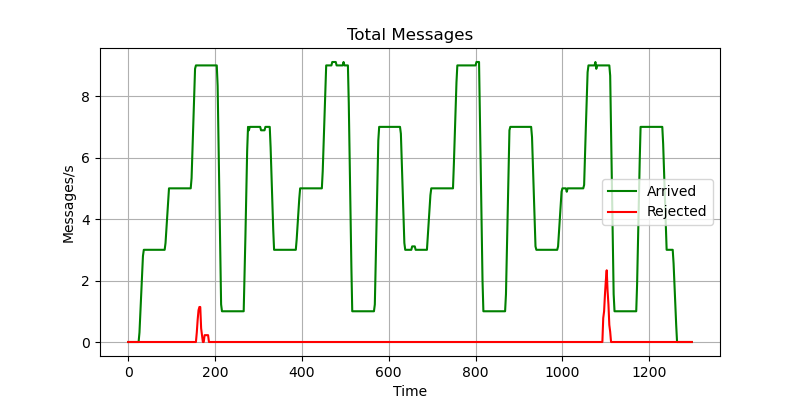
\includegraphics[width=0.85\linewidth]{images/default/constant/messages.png}
	    \caption{Arrived and Rejected messages per second to the Queue.}
	    \label{fig:uniform_messages}
	\end{subfigure}
	\begin{subfigure}{0.85\linewidth}
	    \centering
    		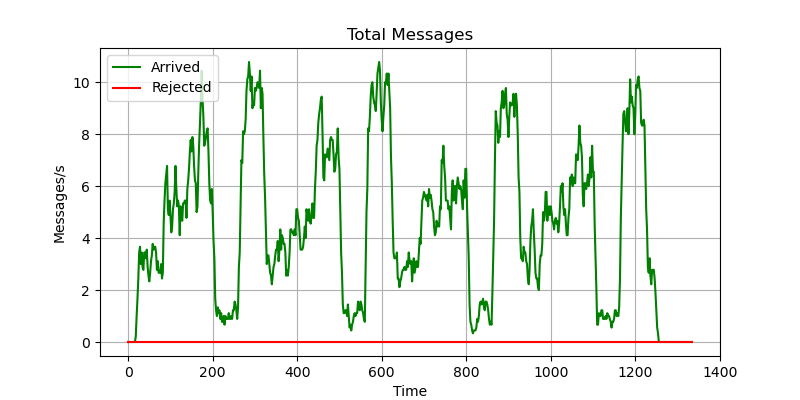
\includegraphics[width=0.85\linewidth]{images/default/exponential/messages.png}
	    \caption{Arrived and Rejected messages per second to the Queue.}
    		\label{fig:uniform_messages}
	\end{subfigure}
\end{figure}
As said, the goal of the control is to keep a rejection rate below 5\%. In figure \ref{fig:uniform_rejection} is reported the cumulative rejection rate through time. To obtain this graph, we calculated the cumulative quantity of rejected messages, and then divided for the corresponding cumulative value of arrived messages. The exact final rejection rate is \textbf{2.8\%}.

\begin{figure}[H]
    \centering
    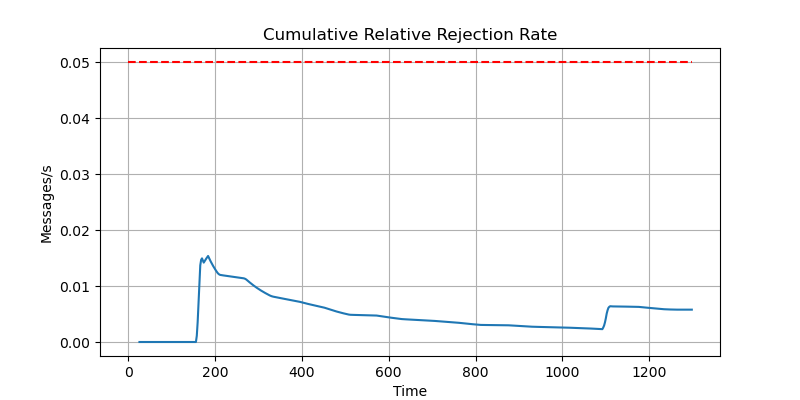
\includegraphics[width=0.85\linewidth]{images/default/constant/rejection_cumulative.png}
    \caption{Cumulative rejection rate.}
    \label{fig:uniform_rejection}
\end{figure}

We can see the rise in rejections after increasing the amount of arriving messages, but after that a descent below the specified target.

Another measure that we consider relevant is the cost inefficiency of the scaler implementation. Due to the fact that creating and destructing pods isn't an immediate operation, Kubernetes takes some time to set the number of replicas to the number prescribed by the Sirio Scaler. This lag in control can be appreciated in figure \ref{fig:uniform_pods}.
\begin{figure}[H]
    \centering
    \begin{subfigure}{0.85\textwidth}
        \centering
        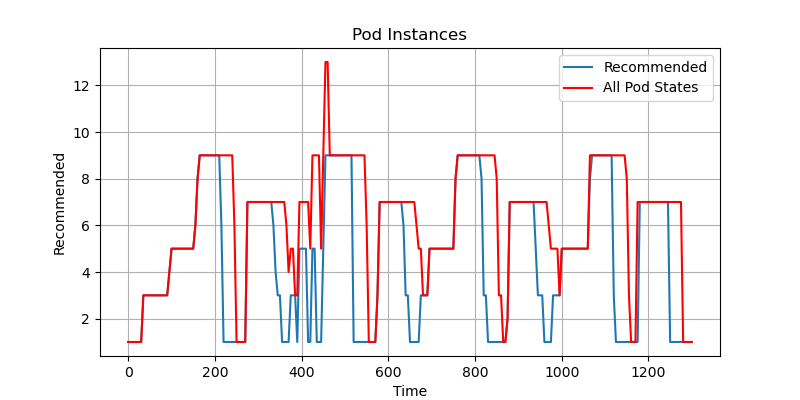
\includegraphics[width=\textwidth]{images/default/constant/pods.png}
        \caption{In blue the number of pods prescribed by the scaler, the red one pods in all states.}
        \label{fig:uniform_pods}
    \end{subfigure}
    \begin{subfigure}{0.85\textwidth}
        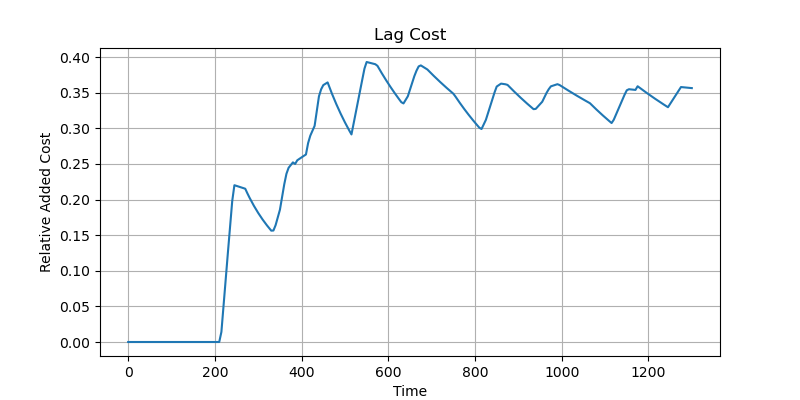
\includegraphics[width=\linewidth]{images/default/constant/lag_cost_cumulative.png}
        \caption{At every time $t$, we calculate the inefficiency from starting time.}
        \label{fig:uniform_inefficiency}
    \end{subfigure}
\end{figure}

In figure \ref{fig:uniform_inefficiency} is reported the inefficiency while the system goes; in the followings more details in how this curve is calculated. To understand this calculation, we need to start from how cost is defined. We choose to measure cost without loss of generality in the unit of $pods \cdot time$, so that the cost of the system is both proportional to the quantity of resources used and the time we used. It's worth noting that this type of billing is common in many types of cloud providers. For example, a system that executes 5 pods for 3 seconds has a cost of 15. So, given any sequence of measured pods $pods_i$ for $i=1,\dots,t$, with a sampling period of $T_s$, the total cost of the system is calculated as \ref{eq:cost}:
\begin{equation}
    \label{eq:cost}
    C = T_s\sum_{i=1}^{t}pods_i
\end{equation}

So, be $C_{preb}$ the prescribed cost obtained by the sequence of pods dictated by the Sirio Scaler, and $C_{real}$ the real cost of all existing pods, we calculated the relative inefficiency as in equation \ref{eq:inefficiency}:
\begin{equation}
    \label{eq:inefficiency}
    I =\frac{C_{real} - C_{preb}}{C_{preb}} = \frac{C_{real}}{C_{preb}} - 1
\end{equation}

Giving the formulas in \ref{eq:cost} and \ref{eq:inefficiency}, both can be calculated for a particular time $t_0$ by truncating the sequence $pods_i$ for $i\leq t_0$.

Note that for how we defined $I$, it can be smaller than 1 in theory. In practice, we consider initializing pods for the actual cost, and making that it's very unlikely that Kubernetes waits so much to start creating them, this eventuality is negligible. However, in equation \ref{eq:inefficiency} we can force the numerator to be bigger or at least equal to the denominator.

We want to state that this measure of inefficiency not necessary means a bad implementation, but only a measure of the difference between a perfect control and the actual one. In fact, this isn't calculated in reference to a commonly used control or any other type.

\subsubsection{Sliding Window}
We also decided to test the system with a state machine composed by exponential distributions. In this case, the states of the machine are associated with these parameters: 2,5 and 10 (The expected value of messages per second in this state are the same). 

The result in terms of arrived and rejected messages is reported in figure \ref{fig:exponential_fast_messages}, and with it the rejection rate in figure \ref{fig:exponential_fast_rejection}:

\begin{figure}[H]
    \centering
    \begin{subfigure}{0.85\linewidth}
        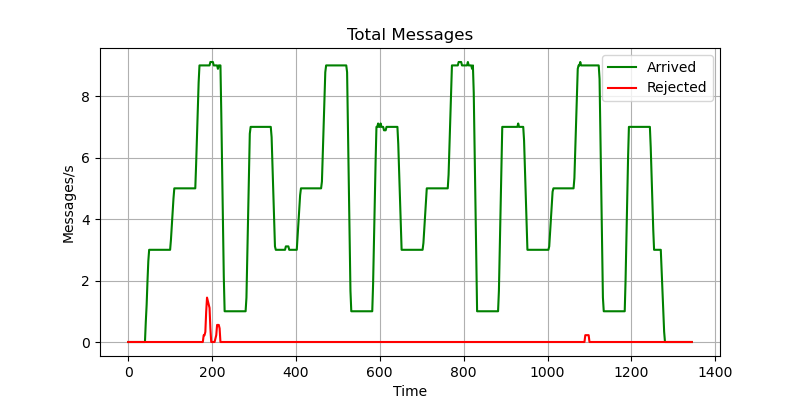
\includegraphics[width=\linewidth]{images/sliding_window/constant/messages.png}
        \caption{Arrived and Rejected messages per second to the Queue.}
        \label{fig:exponential_fast_messages}
    \end{subfigure}
    \begin{subfigure}{0.85\linewidth}
        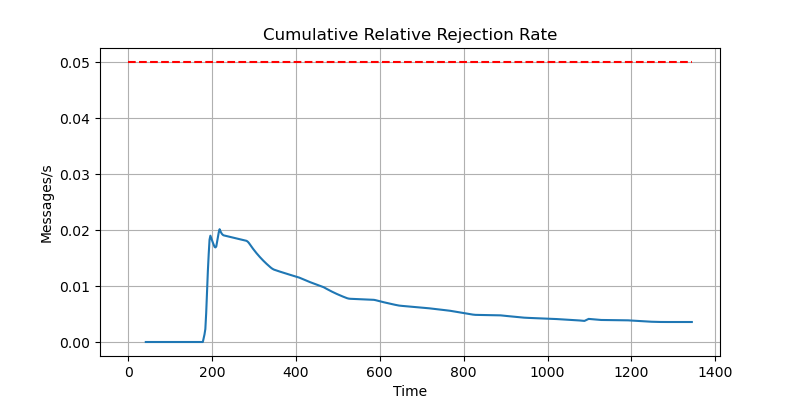
\includegraphics[width=\linewidth]{images/sliding_window/constant/rejection_cumulative.png}
        \caption{Cumulative rejection rate.}
        \label{fig:exponential_fast_rejection}
    \end{subfigure}
\end{figure}
In this case, the surge in rejection came later. This explains why the peak is much lower. In the end, the final rejection rate is \textbf{1.86\%}.

As we can see in figure \ref{fig:exponential_fast_inefficiency}, that the inefficiency in the case of the exponential is greater, even if confronted with the \textit{equivalent} (in terms of expected values of messages per second in the states) uniform case. 

\begin{figure}
    \centering
    \begin{subfigure}{0.85\textwidth}
        \centering
        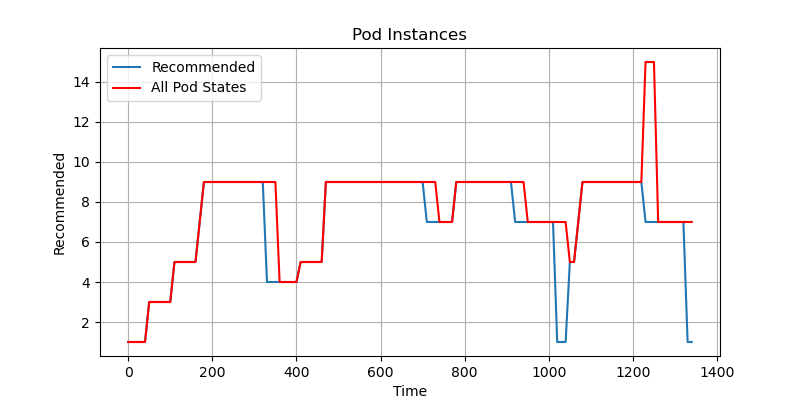
\includegraphics[width=\textwidth]{images/sliding_window/constant/pods.png}
        \caption{In blue the number of pods prescribed by the scaler, the red one pods in all states.}
        \label{fig:exponential_fast_pods}
    \end{subfigure}
    \begin{subfigure}{0.85\textwidth}
        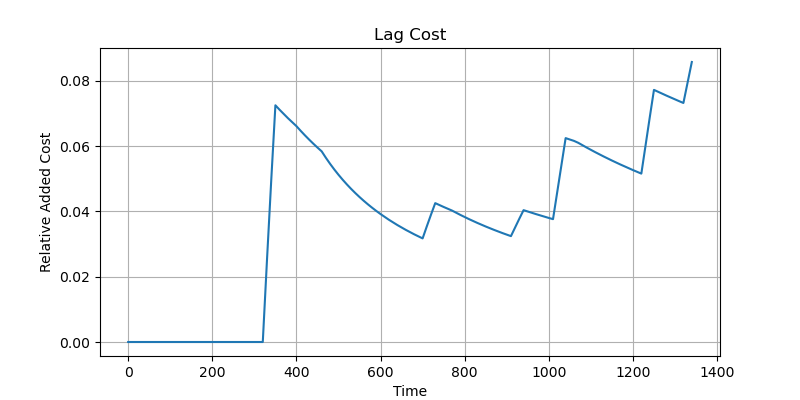
\includegraphics[width=\linewidth]{images/sliding_window/constant/lag_cost_cumulative.png}
        \caption{At every time $t$, we calculate the inefficiency from starting time.}
        \label{fig:exponential_fast_inefficiency}
    \end{subfigure}
\end{figure}

A possible reason for a greater inefficiency can be found in the variance of the stochastic process. In fact, a uniform with the maximum and minimum parameter equal (so a deterministic inter-arrival) has zero variance. In this scenario, Sirio Scaler should not change the prescribed replicas. In the other hand, having an instantaneous (or an average in a short time period) messages arrived per second can make the Sirio Scaler change a little the prescription. So, due to creation or terminating time we have slightly more pods than required.

\section{Conclusions}

In this experimentation we developed a system with microservices, with the aim to verify the feasibility of scaling a workload using stochastic properties of the arrival and service process. We developed a scaling system that models using Sirio framework, and uses its quantitative evaluation for an informed scaling mechanism (in our case funded on rejection rate).

We found that supposing to approximate the arrival process with an exponential form is effective even in the case of a deterministic inter-arrival time, something positive considering how easily we can analyze Markovian systems. Even considering the impossibility to use Bernstein phase types due to their high resource used, we believe that the major precision is not compensating a heavier execution.

In fact, we argue that for arrival processes with a high number of messages per second (condition  that this type of scaling are design for) the shape is not so relevant. So, it's better to have an easier model to obtain quick result to be more reactive.

Another thing to consider is that, for rejection rates target so low, practically the system prescribe a number of service replicas such that the composed rate of service matches the arrival rate. Even if this can conclude in favor of an even simpler solution, the real main advantage of a stochastic approach is the flexibility of the system. We strongly advocate for a use of the Sirio Framework oriented to transient analysis instead of steady state. With this objective in mind, it's trivial to think, as a future development, a scaler that exploits the number of elements in the queue to forecast rejection rate within a short period of time. So to lower the number of replicas even further with a low queue.

In conclusion, we show the feasibility of a horizontal scaling using informed stochastic model, placing the base for further developments.

\appendix
\section{Lag Cost}
\label{sec:lag_cost}
In figure \ref{fig:uniform_inefficiency} is reported the inefficiency while the system goes; in the followings more details in how this curve is calculated. To understand this calculation, we need to start from how cost is defined. We choose to measure cost without loss of generality in the unit of $pods \cdot time$, so that the cost of the system is both proportional to the quantity of resources used and the time we used. It's worth noting that this type of billing is common in many types of cloud providers. For example, a system that executes 5 pods for 3 seconds has a cost of 15. So, given any sequence of measured pods $pods_i$ for $i=1,\dots,t$, with a sampling period of $T_s$, the total cost of the system is calculated as \ref{eq:cost}:
\begin{equation}
    \label{eq:cost}
    C = T_s\sum_{i=1}^{t}pods_i
\end{equation}

So, be $C_{preb}$ the prescribed cost obtained by the sequence of pods dictated by the Sirio Scaler, and $C_{real}$ the real cost of all existing pods, we calculated the relative inefficiency as in equation \ref{eq:inefficiency}:
\begin{equation}
    \label{eq:inefficiency}
    I =\frac{C_{real} - C_{preb}}{C_{preb}} = \frac{C_{real}}{C_{preb}} - 1
\end{equation}

Giving the formulas in \ref{eq:cost} and \ref{eq:inefficiency}, both can be calculated for a particular time $t_0$ by truncating the sequence $pods_i$ for $i\leq t_0$.

Note that for how we defined $I$, it can be smaller than 1 in theory. In practice, we consider initializing pods for the actual cost, and making that it's very unlikely that Kubernetes waits so much to start creating them, this eventuality is negligible. However, in equation \ref{eq:inefficiency} we can force the numerator to be bigger or at least equal to the denominator.

We want to state that this measure of inefficiency not necessary means a bad implementation, but only a measure of the difference between a perfect control and the actual one. In fact, this isn't calculated in reference to a commonly used control or any other type.
\nocite{*}
%\bibliographystyle{plain}
%\bibliography{chapters/Bibliografy}

\end{document}
% -----------------------------------------------------------------
